\documentclass[12pt]{article}

\textheight=24cm %высота текста
\textwidth=16cm %длина текста
\oddsidemargin=0pt %отступ от левого края
\topmargin=-1.5cm %отступ от верхнего края
\flushbottom %выравнивание высоты страниц

\usepackage[utf8]{inputenc}
\usepackage[T2A]{fontenc}

\usepackage{tikz}

\usepackage{amsmath}

\usepackage[russian]{babel}

\title{СВТ. Отчет по заданию 2.1.}
\author{Чаплыгин Андрей}
\date{}

\begin{document}

\maketitle

\section{Вариант задания}

Рассматривается стационарное уравнение диффузии

$$ -\nabla D \nabla C = f $$

в области $\Omega \in R^2$ с границей $\partial \Omega$. $C$ — концентрация вещества, $f = f(x, y)$
— функция источников или стоков. Граница $\partial \Omega$ состоит из
двух частей: $\partial \Omega = G_D \bigcup G_N$, на $G_D$ заданы граничные условия типа
Дирихле, а на $G_N$ — граничные условия типа Неймана, $D = diag(1, \varepsilon)$ - тензор
диффузии.

\bigskip
Вариант 3, МКР.


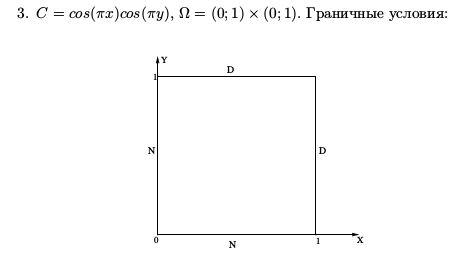
\includegraphics[scale = 0.6]{./task.png}


\section{Результаты}

Метод решения линейной системы - метод сопряженных градиентов SLPCG (Ani2d).

Аппроксимация граничных условий типа Неймана вторым порядком точности:

$\varepsilon = 1 $
\begin{center}
    \begin{tabular}{c|c|c|c}
      \hline
      $h$ & $C_h$ &  $L_h$ &  Число итераций \\
      \hline
      1/32 & 1.0975E-003 & 9.3731E-004 & 47 \\ 
      \hline
      1/64 & 2.7436E-004 & 2.3436E-004 & 71 \\ 
      \hline
	  1/128 &  6.8531E-005 & 5.8583E-005 & 137 \\
	  \hline 
    \end{tabular}
\end{center}

$\varepsilon = 10 $
\begin{center}
    \begin{tabular}{c|c|c|c}
      \hline
      $h$ & $C_h$ &  $L_h$ &  Число итераций \\
      \hline
      1/32 &   1.3421E-003  & 8.9681E-004 & 40 \\ 
      \hline
      1/64 &   3.3530E-004   & 2.2412E-004 & 77 \\ 
      \hline
	  1/128 &  8.3818E-005  & 5.6025E-005 & 149 \\ 
	  \hline 
    \end{tabular}
\end{center}


$\varepsilon = 100 $
\begin{center}
    \begin{tabular}{c|c|c|c}
      \hline
      $h$ & $C_h$ &  $L_h$ &  Число итераций \\
      \hline
      1/32 &   1.5693E-003  & 8.8734E-004  & 27  \\ 
      \hline
      1/64 &   3.9255E-004  & 2.2163E-004  & 52  \\ 
      \hline
	  1/128 &  9.8921E-005  & 5.5346E-005  & 97  \\ 
	  \hline 
    \end{tabular}
\end{center}


Аппроксимация граничных условий типа Неймана первым порядком точности:

$\varepsilon = 100 $
\begin{center}
    \begin{tabular}{c|c|c|c}
      \hline
      $h$ & $C_h$ &  $L_h$ &  Число итераций \\
      \hline
      1/32 &  0.1552  & 5.4932E-002 & 26 \\ 
      \hline
      1/64 &  7.7700E-002  & 2.7543E-002  & 51 \\ 
      \hline
	  1/128 &   3.8868E-002  & 1.3783	E-002 & 96 \\
	  \hline 
    \end{tabular}
\end{center}

\bigskip
\bigskip
На рисунках решение аналитическое, на сетке с N=128, на сетке с N=64 соответственно.

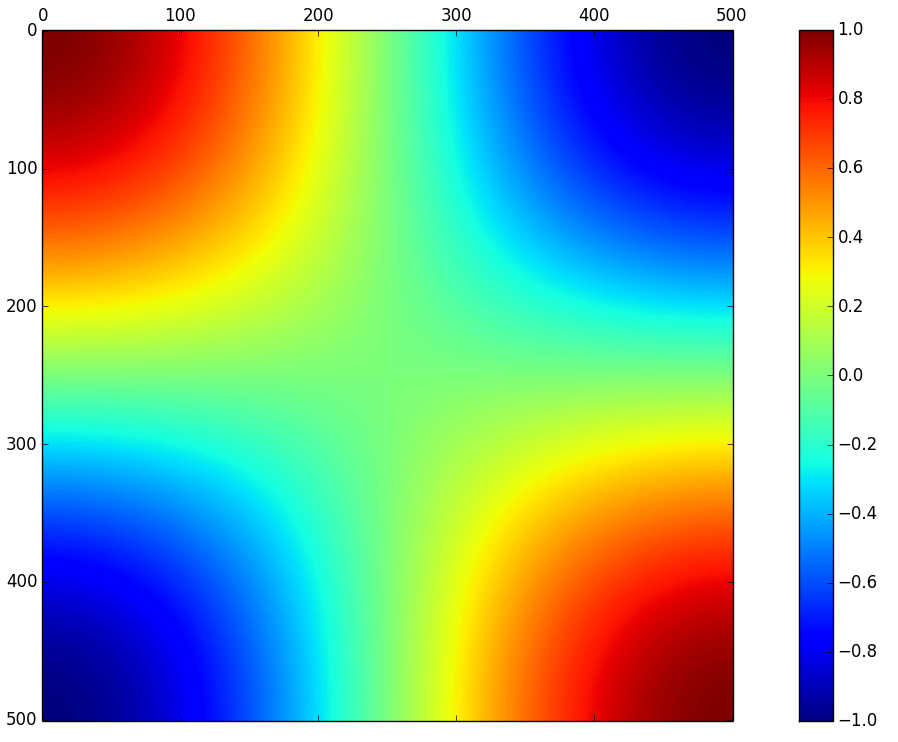
\includegraphics[scale = 0.3]{./solD.png}
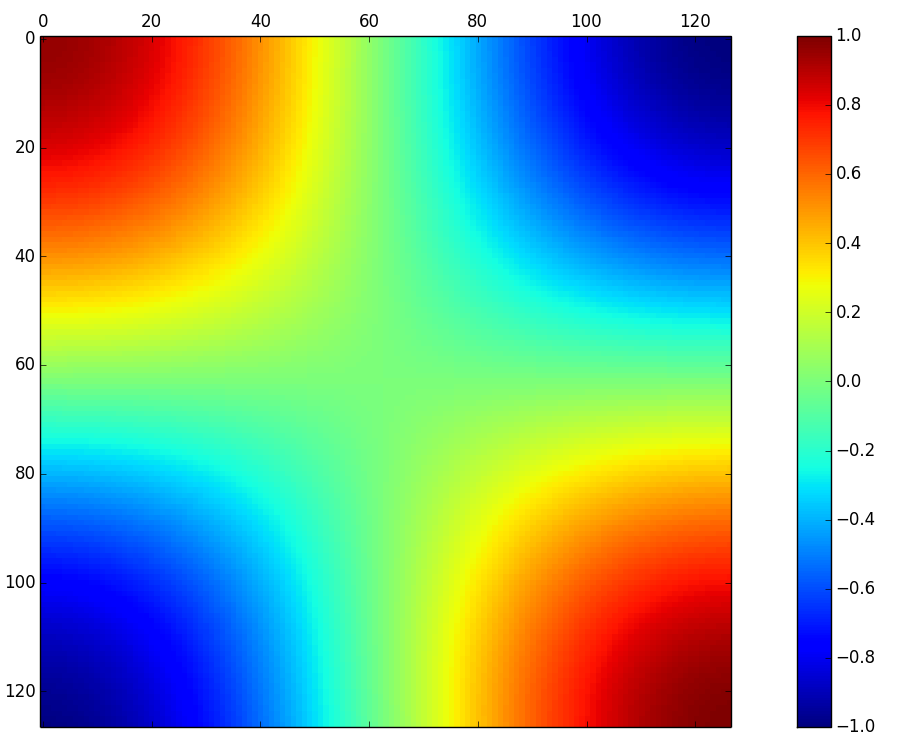
\includegraphics[scale = 0.3]{./numD128.png}

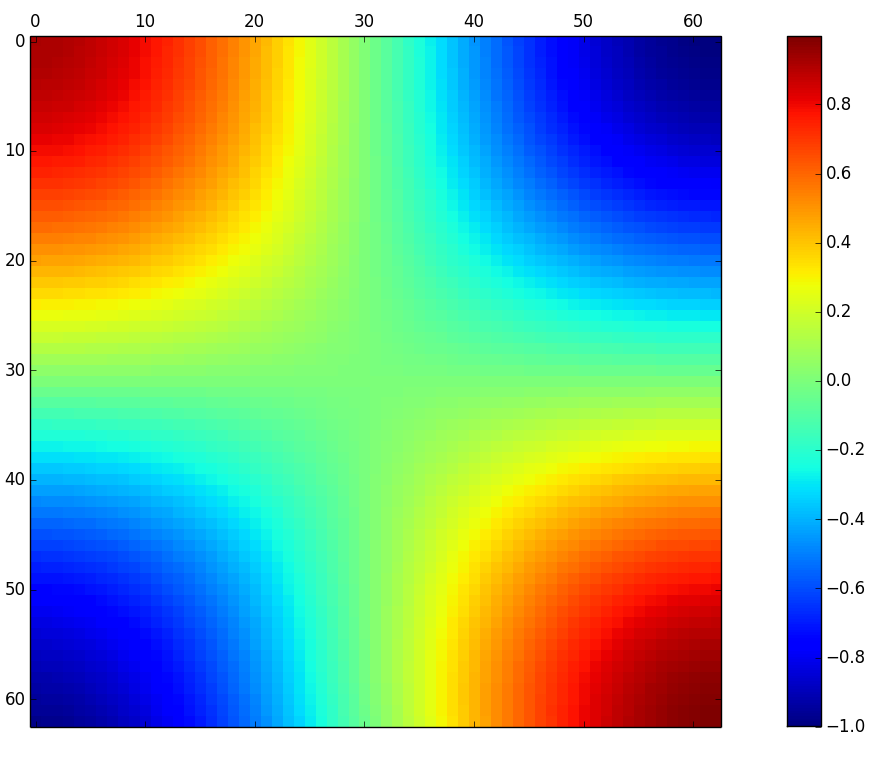
\includegraphics[scale = 0.3]{./numD64.png}



\end{document}
